\section{Basic feasible solutions}

Thanks to the fundamental theorem of linear programming, solving any linear program involves examining the vertices of the polyhedron $P$ containing feasible solutions.
However, because the geometric definition of a vertex isn't suitable for algorithmic use, we require an algebraic characterization.
\begin{example}
    Consider the following linear program:
    \begin{align*}
        \min                      \:&\: -x_1-3x_2          \\
        \textnormal{such that }     &\: x_1+x_2 \leq 6  \\
                                    &\: 2x_1+x_2 \leq 8  \\
                                    &\: x_1,x_2 \geq 0
    \end{align*}
    Its graphical representation is shown below:
    \begin{figure}[H]
        \centering
        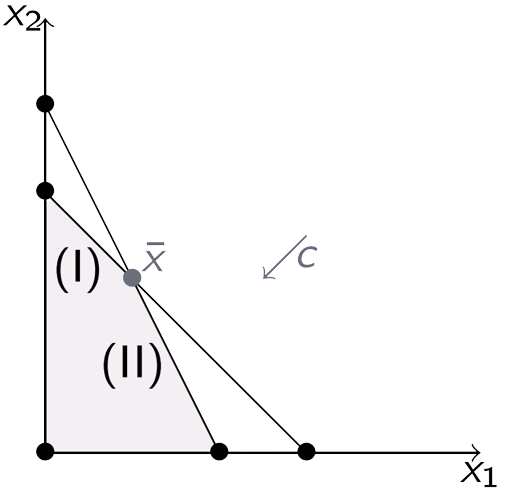
\includegraphics[width=0.25\linewidth]{images/lp.png}
    \end{figure}
    From the graph, it's evident that a vertex corresponds to the intersection of the hyperplanes associated with $n$ inequalities. 
    In this example, the vertex $\overline{x}$ represents the intersection of the first two inequalities, which is the solution to the following system:
    \[
    \begin{cases}
        x_1+x_2=6 \\
        2x_1+x_2=8
    \end{cases}
    \]
    To convert this problem into standard form, we formulate it as:
    \begin{align*}
        \min                      \:&\: -x_1-3x_2          \\
        \textnormal{such that }     &\: x_1+x_2+s_1 = 6  \\
                                    &\: 2x_1+x_2+s_2 = 8  \\
                                    &\: x_1,x_2,s_1,s_2 \geq 0
    \end{align*}
    To solve it, we set $s_1=s_2=0$ and solve the system found before.
    Using this formulation, we can compute all the intersections with the axes:
    \begin{enumerate}
        \item $x_1=0,x_2=0 \rightarrow s_1=6,s_2=8$
        \item $x_1=0,s_1=0 \rightarrow x_2=6,s_2=2$
        \item $x_1=0,s_2=0 \rightarrow x_2=8,s_1=-2$
        \item $x_2=0,s_1=0 \rightarrow x_1=6,s_2=-4$
        \item $x_2=0,s_2=0 \rightarrow x_1=4,s_1=2$
        \item $s_1=0,s_2=0 \rightarrow x_1=2,x_2=4$
    \end{enumerate}
    Note that solutions three and four are infeasible since the values of $s_1$ and $s_2$ are negative. 
\end{example}
\begin{property}
    For any polyhedron $P = \{x \in \mathbb{R}^n|Ax = b,x \geq 0\}$ the facets (equivalent to edges in $\mathbb{R}^2$) are determined by setting one variable to 0. 
\ed{property}
\begin{property}   
    For any polyhedron $P = \{x \in \mathbb{R}^n|Ax = b,x \geq 0\}$ the vertices are determined by setting $n-m$ variables to 0. 
\end{property}

When dealing with a matrix  $A \in \mathbb{R}^{m \times n}$ where $m \leq n$, we can make the following observations:
\begin{itemize}
    \item If $m=n$, there is a unique solution of $Ax = b$.
    \item If $m<n$, there are infinitely many solutions to $Ax = b$. 
        In this case the system has $n-m$ degrees of freedom. 
        As a result $n-m$ variables can be set arbitrarily. 
\end{itemize}
\begin{definition}[\textit{Basis of a matrix}]
    A basis of a matrix $A \in \mathbb{R}^{m \times n}$ containing $n$ variables and $m$ coefficients consists of a subset of $m$ columns from $A$. 
    These columns are linearly independent and collectively form an $m \times m$ non-singular matrix denoted as $B$. 
\end{definition}
Using the earlier definition, we can rearrange the columns of matrix $A$ and then split it to identify the basis as follows:
\[A=\left[ B|N \right]\]
In this partition, $B$ represents an $m \times m$ matrix, and $N$ is a $(n-m) \times m$ matrix.

Let $x^T=\left[x_B^T | x_N^T\right]$, where $x_B^T$ contains  $m$ components and $x_N^T$ contains  $m-n$ components. 
Then, any system $Ax = b$ can be expressed as:
\[Bx_B+Nx_N=b\]
For any given set of values for $x_N$, if matrix  $B$ is non-singular, we can compute $x_B$ as:
\[x_B=B^{-1}b-B^{-1}Nx_N\]
\begin{definition}[\textit{Basic solution}]
    A basic solution is a solution obtained by setting $x_N=0$ and, consequently, letting $x_B=B^{-1}b$.
\end{definition}
\begin{definition}[\textit{Basic feasible solution}]
    A basic solution with $x_B \geq 0$ is a basic feasible solution.
\end{definition}
\begin{definition}[\textit{Basic variables}]
    The variables in $x_B$ are the basic variables.
\end{definition}
\begin{definition}[\textit{Non-basic variables}]
    The variables in $x_N$ are the non-basic variables.
\end{definition}
\begin{theorem}
    An $x \in \mathbb{R}^n$ is a basic feasible solution if and only if $x$ is a vertex of the polyhedron:
    \[P=\{x \in \mathbb{R}^n|Ax=b,x \geq 0\}\]
\end{theorem}
\begin{example}
    In the given linear program:
    \begin{align*}
        \min                      \:&\: 2x_1+x_2+5x_3          \\
        \textnormal{such that }     &\: x_1+x_2+x_3+x_4=4  \\
                                    &\: x_1+x_5=2  \\
                                    &\: x_3+x_6=3 \\
                                    &\: 3x_2+x_3+x_7=6  \\
                                    &\: x_1,x_2,x_3,x_4,x_5,x_6,x_7 \geq 0
    \end{align*}
    The matrices associated with the given constraints are:
    \[
    A=
    \begin{bmatrix}
        1 & 1 & 1 & 1 & 0 & 0 & 0 \\
        1 & 0 & 0 & 0 & 1 & 0 & 0 \\
        0 & 0 & 1 & 0 & 0 & 1 & 0 \\
        0 & 3 & 1 & 0 & 0 & 0 & 1
    \end{bmatrix}
    \:\:\:\:\:\:
    b=
    \begin{bmatrix}
        4 \\
        2 \\
        3 \\
        6
    \end{bmatrix}
    \]
    It can be observed that columns 4, 5, 6, and 7 are linearly independent. 
    By selecting these columns, we obtain:
    \[
    B= 
    \begin{bmatrix}
        1 & 0 & 0 & 0 \\
        0 & 1 & 0 & 0 \\
        0 & 0 & 1 & 0 \\
        0 & 0 & 0 & 1
    \end{bmatrix}
    =I=B^{-1}
    \]
    The solution in this case is $x_B=B^{-1}b=b$, which is a feasible solution.
    However, if we choose columns 2, 5, 6, and 7, the solution is $x_B=\begin{bmatrix} 4 & 2 & 3 & -6 \end{bmatrix}^T$, which is an infeasible solution.
\end{example}
The total number of feasible solutions can be calculated as:
\[\textnormal{number of feasible solutions}=\binom{n}{m}\]